\section{Uni-variate representation of the curves} \label{app:alternativeRep}

\paragraph{Line}
The alternative representation of the level-curve of a linear function $f(x,y)=ax+by+c$ could be written as:

\[
\dot{f}(\theta) = (x,y) =
\begin{cases}
  \left( x_l + \theta, y_l \right) & \quad \text{if } s = 0\\
  \left( x_l, y_l + \theta \right) & \quad \text{if } s = \pm \infty\\
  \left( x_l + \dot{a}\theta , y_l + \dot{b}\theta \right) & \quad \text{otherwise} \\
\end{cases}\\
\]

where $(x_l,y_l)$ is an arbitrary (but fixed as a reference) point on the level-curve of the $f(x,y)$, $s$ is the slope of the level-curve of $f(x,y)$, and $\dot{a}, \dot{b}$ are given by:
\[
\dot{a} = \frac{\sqrt{ s^2 + 1}}{s^2 + 1}, \quad \dot{b} = \dot{a}s
\]

The inverse function ($\theta = \dot{f}^{-1}(x,y)$) is given by:
\[
\theta = \dot{f}^{-1}(x,y) =
\begin{cases}
  x & \quad \text{if } s = 0\\
  y & \quad \text{if } s = \pm \infty\\
  \frac{x-x_l}{\dot{a}} & \quad \text{if } \dot{a} \neq 0\\
  \frac{y-y_l}{\dot{b}} & \quad \text{otherwise} \\
\end{cases}\\
\]

While the second derivative of a line is a null vector, the first derivative of a line in this representation would be:
\[
\begin{array}{l}
  \frac{d\dot{f}(\theta)}{d\theta} = \left( \cos(\theta) , \sin(\theta) \right) \text{, where } \theta = \arctan(s)\\
\end{array}
\]

The angle of the tangent vector to a linear curve

\[
\begin{array}{l}
s = \frac{\Delta y}{\Delta x} = \tan(\theta)\\
\theta = \arctantwo(\Delta y , \Delta x)\\
\end{array}
\]

Linear curvature has a curvature of zero.

\[
\begin{array}{l}
k = \frac{ x'y'' - y'x'' }{ \left(x'^2+y'^2\right)^{\frac{3}{2}}}, (x'', y'') = 0 \quad \rightarrow k = 0\\
\end{array}
\]




%%%%%%%%%%%%%%%%%%%%%%%%%%%%%%%%%%%%%%%%
\paragraph{Circle}
Similarly, for the level-curve of a conic function $f(x,y)=(x-x_c)^2+(y-y_c)^2-r_c$ (hence the level-curve would be a conic section, in this case a circle) the alternative representation can be written as:

\[
\dot{f}(\theta) = (x,y) = \left( x_c + r_c \cos(\theta), y_c + r_c \sin(\theta) \right)
\]

where $(x_c,y_c)$ is the center of the $f(x,y)$ function, and radius $r_c$ defines the desired level-curve of the $f(x,y)$.\bigskip

The inverse function ($\theta = \dot{f}^{-1}(x,y)$) is given by:

\[
\theta = \dot{f}^{-1}(x,y) = \arctantwo (y - y_c, x - x_c)
\]

The first and second derivatives of a circle in this representation are:
\[
\begin{array}{l}
  \frac{d\dot{f}(\theta)}{d\theta} = \left( -r_c \sin(\theta), r_c \cos(\theta) \right)\\
  \quad\\
  \frac{d^2\dot{f}(\theta)}{d\theta^2} = \left( -r_c \cos(\theta), -r_c \sin(\theta) \right)\\
\end{array}
\]

The angle of the tangent vector to a circle at a given point $p$ contained by the circle is:
\[
\begin{array}{l}
\tan(\theta) = \frac{\Delta y}{\Delta x} = \frac{d\dot{f}(\theta)}{d\theta}(p) \\
\theta = \arctantwo(\Delta y , \Delta x)\\
\end{array}
\]

curvature of a circle is the radius' reciprocal.

\[
\begin{array}{l}
k = \frac{ x'y'' - y'x'' }{ \left(x'^2+y'^2\right)^{\frac{3}{2}}}\\
x', y' =  -r_c\sin(\theta), r_c\cos(\theta)\\
x'', y'' = -r_c\cos(\theta), -r_c\sin(\theta) \\
k = \frac{\left(-r_c\sin(\theta) \times -r_c\sin(\theta)\right) - \left(-r_c\cos(\theta) \times r_c\cos(\theta)\right)} {\left(\left(-r_c\sin(\theta)\right)^2 + \left(r_c\cos(\theta)\right)^2\right)^{\frac{3}{2}} } \\
\quad = \frac{ r_c^2\sin^2(\theta) + r_c^2\cos^2(\theta)}{ \left(r_c^2\sin^2(\theta) + r_c^2\cos^2(\theta)\right)^{\frac{3}{2}}} = \frac{r_c^2}{r_c^3} \times \frac{ \sin^2(\theta) + \cos^2(\theta)}{ \left(\sin^2(\theta) + \cos^2(\theta)\right)^{\frac{3}{2}}}\\
\rightarrow k = \frac{1}{r}\\
\end{array}
\]

%%%%%%%%%%%%%%%%%%%%%%%%%%%%%%%%%%%%%%%%
\paragraph{Direction of half-edges and the derivatives}
The half-edges are directed, as the same segment of a curve turns into two half-edges with opposite directions.
Direction of half-edges is very important in the correct calculation of the first derivative vectors.
If a half-edge has a negative direction with respect to the direction of $\theta$, as demonstrated in figure~\ref{fig:appa_derDirection}, its first derivative vectors are rotated $180^o$ degrees to face in the opposite direction.


\begin{figure}%[!ht]
  \centering
  \begin{subfigure}{.8\textwidth}
    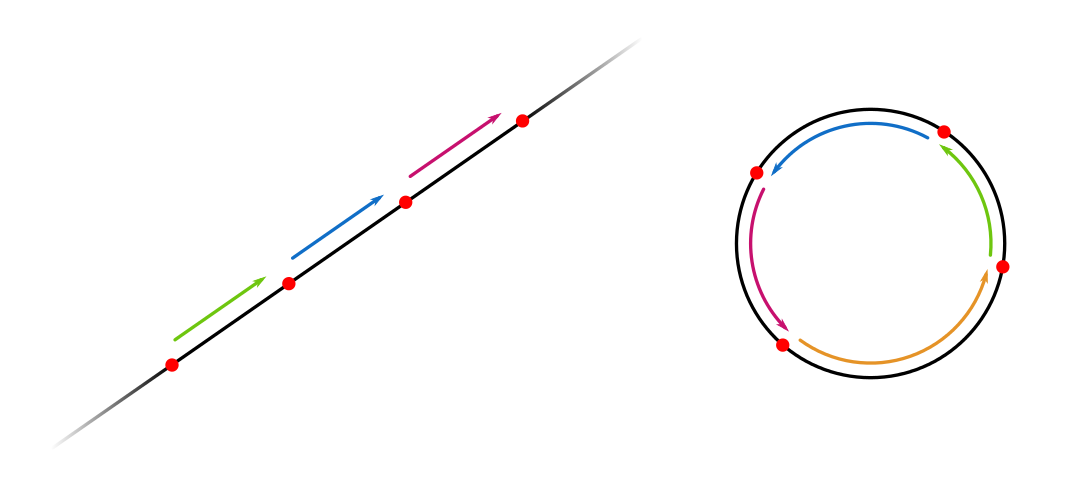
\includegraphics[width=\textwidth]{figures/appa_derDirection_pos.png}
    \caption{half-edges with positive direction} \label{subfig:appa_derDirection_pos}
  \end{subfigure}

  \begin{subfigure}{.8\textwidth}
    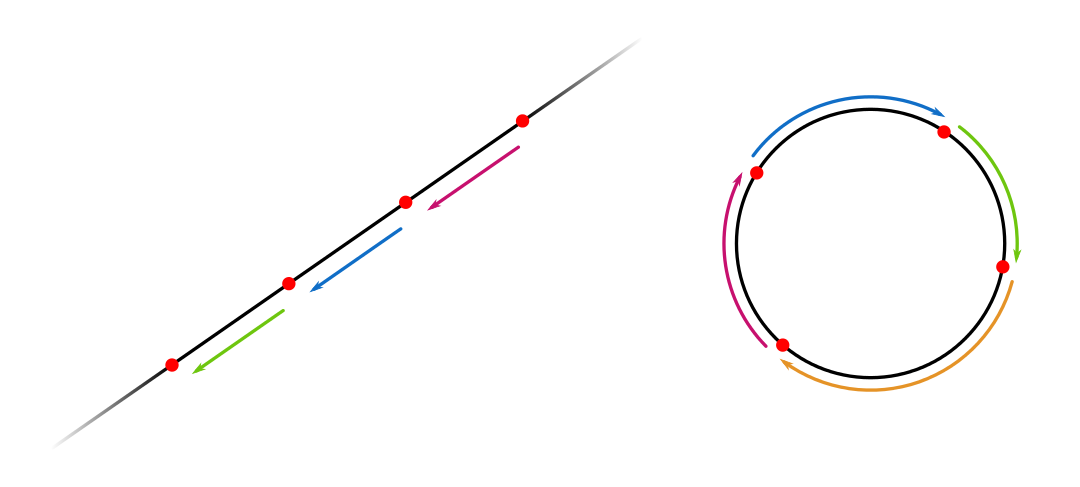
\includegraphics[width=\textwidth]{figures/appa_derDirection_neg.png}
    \caption{half-edges with negative direction} \label{subfig:appa_derDirection_neg}
  \end{subfigure}
  \caption[xxx]
          {Direction of half-edges and its effect on the derivative vectors.}
  \label{fig:appa_derDirection}
\end{figure}



